%% VEGABrain -- manuscript for Neuroinformatics (Springer)
%% Springer Nature journal article template v3.1 (December 2024).
%% Reference style: sn-basic (author-year), which is what Neuroinformatics uses.
%% Build:  bash build.sh      (see IMPLEMENTATION.md)
%%
%% Add the "lineno" option below when producing the copy for reviewers:
%%   \documentclass[lineno,pdflatex,sn-basic]{sn-jnl}

\documentclass[pdflatex,sn-basic]{sn-jnl}

%%%% Standard Packages
\usepackage{graphicx}%
\usepackage{amsmath,amssymb,amsfonts}%
\usepackage{xcolor}%
\usepackage{textcomp}%
\usepackage{manyfoot}%
\usepackage{booktabs}%
\usepackage{url}%
%%%%

\graphicspath{{figures/}}
\raggedbottom

\begin{document}

\title[VEGABrain]{VEGABrain: a Visualizer of Enriched Gene Analysis for the
developing human brain}

%% TODO(authors): confirm author order, add ORCIDs via \orcid{...} inside \author,
%% and replace the affiliation placeholders with the full postal address of the
%% MCB Lab / department at UFRN.

\author[1]{\fnm{Isaac} \sur{Medeiros}}\email{isaac.medeiros.112@ufrn.edu.br}

\author[1]{\fnm{Jo\~{a}o V.} \sur{F. Cavalcante}}\email{joao.cavalcante.073@ufrn.edu.br}

\author*[1]{\fnm{Diego} \sur{Marques-Coelho}}\email{diego.marques.135@ufrn.edu.br}

\affil*[1]{\orgdiv{Bioinformatics Multidisciplinary Environment}, \orgname{Federal University of Rio Grande do Norte}, \orgaddress{\street{Rua do Horto}, \city{Natal}, \postcode{59076-550}, \state{Rio Grande do Norte}, \country{Brazil}}}

%%==================================================================%%
%% Abstract
%%==================================================================%%

\abstract{
  RNA sequencing datasets are widely reused resources in developmental neuroscience, yet inspecting them spatially remains unclear and difficult. Here, we present VEGABrain, an openly accessible web tool that renders bulk RNA-seq onto brain cortical and subcortical atlas surfaces across five human developmental windows spanning the first trimester to adulthood. Beyond single-gene maps, VEGABrain contributes a composite per-region enrichment layer using single-sample gene set enrichment analysis (ssGSEA) scores precomputed for 18{,}650 gene sets drawn from Gene Ontology, Reactome, KEGG, BioCarta, the Human Phenotype Ontology and the MSigDB hallmark collection, and aggregated to a score for every gene set, developmental window and brain region. Furthermore, VEGABrain allows users to submit a custom gene list and obtain its ssGSEA map across development, computed on demand. Submitted lists can also be tested: two complementary per-area tests---one competitive on the ssGSEA score, one for over-representation of area-specific marker genes---mark the regions where a list stands out, and a developmental-stage test reports the windows in which it peaks, for the whole brain and for six major regions. VEGABrain is open source and requires no installation, offering easy-to-query expression throughout development and brain areas.
}

\keywords{Neuroinformatics, Brain development, BrainSpan, Gene set enrichment,
ssGSEA, Data visualization, Web application}

\maketitle

%%==================================================================%%
\section{Introduction}\label{sec:intro}
%%==================================================================%%

The transcriptome of the developing human brain is one of the most heavily
reused datasets in neuroscience. The BrainSpan atlas
\citep{BrainSpan2011,Kang2011,Miller2014} sampled bulk tissue from cortical and
subcortical structures across prenatal and postnatal donors, and subsequent
integrative work built on it to relate developmental expression to
neuropsychiatric risk \citep{Li2018} and to evolutionary divergence between
human and macaque \citep{Zhu2018}.

What has not kept pace is the ease of seeing it. A researcher who wants
to know where and when a gene, or a set of genes, is expressed in the developing
brain has essentially two options today, and both impose costs that are
unrelated to the biological question.

The first is the resource portal. Portals in this family---BrainSpan itself, and
the wider family of Allen Institute browsers \citep{Lau2008,Sunkin2013}---return
the data as tables, line plots or heat maps indexed by structure acronym. This, unfortunately, is 
not anatomical: the reader must hold the mapping from
\texttt{DFC}, \texttt{MFC} or \texttt{STC} to a location in the brain, 
and a heat map of 26 structure codes does not convey a spatial gradient
the way a rendered cortex does. It is also gene-at-a-time. There is no route
from a gene set, a pathway, or the output of a differential-expression analysis
to a spatial view. Newer hosted portals have narrowed part of this gap:
BrainScope links genes and samples through t-SNE maps to choropleths over
anatomical slices \citep{Huisman2017}, and SMDB browses spatial transcriptomic
data in two and three dimensions \citep{Cao2023}. Neither, however, scores a
gene set across a human developmental parcellation
(Section~\ref{sec:comparison}).

The second option would be through brain-plotting
tools as---\texttt{ggseg} and \texttt{ggseg3d} \citep{Mowinckel2020} and
\texttt{cerebroViz} \citep{Bahl2017} in R, \texttt{neuromaps} in Python
\citep{Markello2022}, and \texttt{abagen} for the adult Allen Human Brain Atlas
\citep{Hawrylycz2012,Markello2021}. But that route presupposes a user who
writes R or Python, who is willing to download and hold a $52{,}376 \times 524$
expression matrix locally, and who will construct and validate the mapping from
BrainSpan's tissue nomenclature onto an atlas parcellation. Each of those steps
is a place where a project stalls or a mapping silently diverges between
laboratories \citep{Markello2021}.

Additionally, modern analyses rarely end
with one gene. They end with a list, be it a differentially expressed set, a module
from a co-expression network or a panel of risk genes for a disorder. The natural
question is then not ``where is gene $X$ expressed?'' but ``where and when is
this programme active?''. Answering it requires collapsing many genes
into a single per-sample summary. Single-sample gene set enrichment analysis
(ssGSEA) \citep{Barbie2009}, a per-sample variant of GSEA
\citep{Subramanian2005} implemented alongside GSVA \citep{Hanzelmann2013},
provides exactly such a composite score, and has been used as a quantitative
readout of pathway activity in expression data
\citep{Yi2020}. The incorporation of composite multigene activity scores (such as those generated by ssGSEA or GSVA) into anatomical models directly addresses the challenge of condensing high-dimensional expression profiles into interpretable summaries, ensuring noise reduction and dimensionality reduction compared to classical single-gene-based analyses \citep{Hanzelmann2013}. To our knowledge no tool has applied it as a
\emph{spatial} layer over the developing human brain.

VEGABrain (Visualizer of Enriched Gene Analysis) addresses these three gaps in
one interface, reachable at \url{https://mcblab.github.io/VEGABrain/} with no
installation, account or download. It maps BrainSpan samples onto cortical and
subcortical atlas parcels across five developmental windows; it adds a composite
enrichment layer of ssGSEA scores precomputed for 18{,}650 gene sets from the
Gene Ontology \citep{Ashburner2000,GOConsortium2023}, Reactome
\citep{Gillespie2022}, KEGG \citep{Kanehisa2000}, BioCarta, the Human Phenotype
Ontology \citep{Kohler2021} and the MSigDB hallmark collection
\citep{Liberzon2011,Liberzon2015}; and it scores user-submitted gene lists on
demand, closing the loop from an enrichment result \citep{Chen2013,Kuleshov2016}
back to anatomy. A submitted list may also carry log2 fold-change values from an
external comparison---a different disease model, treatment or condition---which
are then mapped against the BrainSpan expression data, so that analyses can
follow directions the dataset was not originally built for, not just the
comparisons already included in it. A submitted list is also tested
statistically: VEGABrain marks the areas where it stands out against random
genes of the same expression level, and reports the developmental windows in
which it peaks, so that a map can be read as a result rather than only as a
picture. Both the maps and the numbers behind them are exportable, so
that VEGABrain is a starting point for downstream analysis, 
consistent with reusable research data
\citep{Wilkinson2016}.

%%==================================================================%%
\section{Materials and Methods}\label{sec:methods}
%%==================================================================%%

\subsection{Expression data and preprocessing}\label{sec:data}

VEGABrain is built on the BrainSpan Developmental Transcriptome RNA-Seq release,
Gencode v10 RPKM values summarised to genes \citep{BrainSpan2011,Li2018}.
The distributed matrix contains 52{,}376 gene rows and 524 sample columns. Rows
with duplicate HGNC symbols are dropped, keeping the first occurrence, and
values are transformed as $\log_2(\mathrm{RPKM} + 1)$. No further normalisation
or batch correction is applied; the released RPKM values are used as the
provider distributes them, so that scores computed here remain comparable with
analyses performed directly on the public matrix. Preprocessing and the scoring
described in Section~\ref{sec:ssgsea} are performed once, offline
(Figure~\ref{fig:arch}).

\subsection{Developmental windows}\label{sec:ages}

BrainSpan donors span 31 distinct ages from 8 post-conceptional weeks (pcw) to
40 years. Individual ages are too sparsely sampled to render as separate maps,
so donors are binned into five developmental windows: first trimester (8--12
pcw, $n=5$ donors), second trimester (13--21 pcw, $n=10$), third trimester
(24--37 pcw, $n=5$), child ($n=14$) and adult ($n=8$).

The two postnatal windows split the postnatal donors at 18 years, where
BrainSpan's sampling has a natural gap: no donor is aged between 15 and 18
years. The child window therefore holds every postnatal donor under 18: 14
donors aged 4 months to 15 years, five of them under two years, four aged 2 to
4 years and five aged 8 to 15 years. It spans infancy, childhood and
adolescence (periods 8--12 of \citealp{Kang2011}), so a result in this window
describes the maturing postnatal brain as a whole rather than any one of those
stages. The adult window holds the eight donors aged 18 to 40
years, one per age, four male and four female. No donor is older than 40, so
this window covers young adulthood and says nothing about ageing.

The donor counts and age ranges are also given in Table~\ref{tab:data}; the
donor count is displayed in every facet label in the
interface so that the reader is never shown a map without also being shown how
much evidence stands behind it.

\subsection{Mapping BrainSpan structures to an atlas}\label{sec:mapping}

BrainSpan labels tissue by dissected structure (for example \emph{dorsolateral
prefrontal cortex}), whereas \texttt{ggseg} draws atlas parcels (for example
\emph{rostral middle frontal}). Cortical regions map onto the Desikan--Killiany parcellation
\citep{Desikan2006} and subcortical structures onto the FreeSurfer
\texttt{aseg} segmentation \citep{Fischl2002}, both accessed through
\texttt{ggseg} \citep{Mowinckel2020}.

Each atlas parcel takes the samples of one BrainSpan structure, except the
thalamus and the cerebellum, which pool the two names BrainSpan gives each
(dorsal thalamus and mediodorsal nucleus of the thalamus; cerebellum and
cerebellar cortex). BrainSpan samples far fewer structures than the atlases
draw, so the assignment is many-to-one: 22 of BrainSpan's 26 structures cover
28 atlas parcels---21 of the 34 Desikan--Killiany cortical parcels and seven
\texttt{aseg} structures (amygdala, hippocampus, thalamus, caudate, putamen,
nucleus accumbens and cerebellum)---and parcels that fall within one dissected
structure share its value (for example, the rostral and caudal middle frontal
parcels both take the dorsolateral prefrontal cortex samples, and the caudate,
putamen and nucleus accumbens all take the striatum samples). The four
structures left out, the medial, lateral and caudal ganglionic eminences and
the upper rhombic lip, are transient fetal structures with no counterpart in
either atlas. Atlas parcels with no BrainSpan counterpart are left unassigned
and drawn in grey: 13 Desikan--Killiany parcels, among them the superior
frontal gyrus, insula, precuneus and fusiform gyrus, and \texttt{aseg}
structures such as the brain stem, pallidum and choroid plexus. The complete assignment is a single
table, provided as Supplementary File~1 and read by the application as is, so
it can be inspected and changed rather than reimplemented per project.

The interface exposes two levels of granularity. At the \emph{micro} scale each
of the 28 mapped atlas parcels carries its own value. At the \emph{macro} scale
regions are pooled into six anatomical groupings---frontal, parietal, temporal
and occipital lobes, subcortical structures and cerebellum---the mean is taken
within each grouping, and that mean is painted back onto every region belonging
to it. The macro scale exists because BrainSpan sampling density varies sharply
across structures: pooling trades spatial resolution for donor support, and
letting the user switch between the two makes that trade-off explicit rather
than hidden. Regions with no corresponding sample are drawn in grey rather than
imputed.

Every map is rendered as four stacked panels---right lateral cortex, right
medial cortex, subcortical sagittal and subcortical coronal---each faceted into
the five developmental windows, giving a single figure in which spatial and
temporal structure are read on orthogonal axes.

\subsection{Composite enrichment scores}\label{sec:ssgsea}

For a gene set $G$ and a sample $j$, ssGSEA \citep{Barbie2009} ranks all genes
by their expression within that sample and computes an enrichment score from
the normalised difference between the empirical cumulative distribution of the
genes in $G$ and that of the genes outside it:

\begin{equation}\label{eq:ssgsea}
\mathrm{ES}(G, j) \;=\;
\sum_{i=1}^{N}\Bigl( P^{G}_{\mathrm{w}}(G, j, i) - P^{NG}(G, j, i) \Bigr),
\end{equation}

where $i$ indexes genes in decreasing order of expression in sample $j$,
$P^{G}_{\mathrm{w}}$ is the weighted cumulative distribution over genes in the
set and $P^{NG}$ the cumulative distribution over the rest. Because the score is
computed from within-sample ranks, it is invariant to the monotone
transformation applied in Section~\ref{sec:data} and does not require a
reference group or a phenotype contrast---which is what makes it usable here,
where each sample is a single donor--structure pair rather than a member of a
case/control design. We use the \texttt{ssgseaParam} interface of the
\texttt{GSVA} package \citep{Hanzelmann2013} with default parameters.

Gene sets are retrieved through \texttt{msigdbr} \citep{Dolgalev2026msigdbr} for
\emph{Homo sapiens} and comprise the MSigDB hallmark collection
\citep{Liberzon2015}, the canonical pathway subcollections BioCarta, KEGG
\citep{Kanehisa2000} and Reactome \citep{Gillespie2022}, and the full C5
ontology collection, which supplies Gene Ontology biological process, molecular
function and cellular component terms \citep{Ashburner2000,GOConsortium2023}
together with Human Phenotype Ontology terms \citep{Kohler2021}. The resulting
18{,}650 sets are broken down by collection in Table~\ref{tab:data}.

Scores are computed once for every gene set against all 524 samples, then
aggregated: for each (gene set, developmental window, region) triple the mean
score over the contributing samples is stored, and analogously for macro-regions,
so that an ontology query needs no enrichment run at request time. When instead a user submits their own gene list, the symbols are validated
against the matrix (unmatched symbols are reported back rather than silently
dropped), ssGSEA is run for that single set across all samples, and the same
aggregation is applied before rendering.

\subsection{Significance testing for gene lists}\label{sec:tests}

A map shows where a score is high; it does not say whether that is more than
chance. For a submitted list, VEGABrain therefore offers three tests, run on
request and reported on the map and in the exported table
(Table~\ref{tab:tests}). All three are computed from the expression matrix and
its sample annotation at request time, with no precomputed reference. The unit
of inference is always the BrainSpan structure or region class, never the atlas
parcel: results are painted onto parcels only for display, because parcels fed
by the same structure carry the same measurement (Section~\ref{sec:mapping}).

\paragraph{Score test.} It asks whether the list, taken as a whole, is more
active in a structure than in the other structures sampled in the same window.
For every structure--window cell with at least three donors (70 of 87 cells),
the list's mean ssGSEA score is taken as its deviation from the mean over that
window's structures, and this deviation is ranked against those of 4{,}000
random gene sets of the same size, each gene replaced by one from the same bin of
mean expression (50 bins over the MSigDB gene universe). Centring within the
window is what makes the test spatial: without it, any list with a developmental
trend would mark every structure of its peak window. $p$-values are corrected by
the Benjamini--Hochberg procedure over all tested cells \citep{Benjamini1995},
and a cell is reported only if it stays below $0.05$ when each of its donors is
left out in turn. For a list with log2FC values the score is the
weight-averaged $z$-score of its genes, and the random sets carry the same
weights. So that 4{,}000 random sets can be scored per request, ssGSEA is
computed from per-sample rank tables built once; this reproduces \texttt{GSVA}
to a relative error below $2 \times 10^{-5}$.

\paragraph{Marker test.} It asks whether the list contains the genes that set an
area apart, following the logic of tissue- and cell-type-specific expression
analysis \citep{Dougherty2010,Xu2014}. In each window, \texttt{limma}
\citep{Ritchie2015} fits expression on structure with donor as a fixed effect,
so that every contrast is made within donors, and tests two levels of contrast:
each of six region classes (neocortex, hippocampus, amygdala, striatum,
thalamus, cerebellum) against the equally weighted mean of the other five, and
each neocortical area against the mean of the other neocortical areas. Genes
with $q < 0.05$, $\log_2$ fold change $\geq 1$ and mean
$\log_2(\mathrm{RPKM}+1) \geq 1$ are that area's markers. A one-sided Fisher
exact test then compares the list with the markers, within the window's
expressed MSigDB genes, with Benjamini--Hochberg correction over all tested
cells. A cell is tested if it has at least 10 markers and three informative
donors (36 cells), and a hit needs $q < 0.05$ and at least two shared genes. A
list with log2FC values is tested separately for its up- and down-regulated
genes. Unlike the score test, the marker test names the user's genes that are
responsible for each hit.

\paragraph{Stage test.} It asks in which window, rather than in which area, a
list stands out---a question the two area tests cannot answer, because both
compare areas within one window. For each window, the list's ssGSEA score is
averaged by structure, then by region class, then over the six region classes
of the PsychENCODE grouping (NCX, HIP, AMY, STR, MD, CBC; \citealp{Li2018}) with
equal weight, so that every window has the same regional make-up even though
BrainSpan sampled different structures at different ages. The window value minus
the list's mean over the five windows is ranked against the same 4{,}000
expression-matched random sets; the test is two-sided, Benjamini--Hochberg
corrected over the windows, and guarded by leaving out each donor of the window
in turn. It is repeated inside each region class, where a region--window cell is
tested only if it has at least three donors; in the third trimester only the
neocortex and the cerebellum qualify. The whole-brain and regional rows are
corrected as separate families, and a list with log2FC values is also tested as
its up- and down-regulated halves.

\paragraph{Calibration.} Each test was run on lists that carry no signal
(Table~\ref{tab:tests}): uniform random lists of 15, 50 and 200 genes,
random lists with log2FC weights, and real MSigDB sets with every gene swapped
for one of matched expression. At most 5\% of such lists produced a single
marked cell in any test. On real MSigDB sets, by contrast, 36\% had a
score-test hit, 15\% a marker-test hit and 44\% a stage-test hit---the last
reflecting that development is the dominant axis of variation in brain
expression, which is why the stage test reports an effect size ($z$) for every
window. Positive controls behaved as expected: eight striatal markers
(\emph{PPP1R1B}, \emph{DRD1}, \emph{DRD2} and others) mapped to the striatum in
all four testable windows and nowhere else, and the astrocyte-development,
myelin-assembly and cell-cycle sets (\texttt{GOBP\_ASTROCYTE\_DEVELOPMENT},
\texttt{GOBP\_MYELIN\_ASSEMBLY}, \texttt{HALLMARK\_G2M\_CHECKPOINT} and
\texttt{HALLMARK\_E2F\_TARGETS}) peaked in the third trimester, after birth and
in the first two trimesters, respectively. Every list used in this work is given
in Supplementary Table~2.

\subsection{Implementation}\label{sec:impl}

VEGABrain is an R \citep{RCoreTeam2026} service built with \texttt{plumber}
\citep{Schloerke2026plumber} behind a browser interface (Figure~\ref{fig:arch}).
Maps are rendered with \texttt{ggplot2} \citep{Wickham2016} and \texttt{ggseg}
\citep{Mowinckel2020}, and can be downloaded as vector (SVG) figures together
with the per-region values behind them as CSV. The same service is exposed as a
public HTTP API, documented in the source repository, so that maps and tables
can also be retrieved programmatically. The significance tests
(Section~\ref{sec:tests}) use \texttt{limma} \citep{Ritchie2015} for the marker
contrasts and are exposed through the same API: a \texttt{significance}
parameter on the gene-list map and table, and two endpoints that return every
tested cell, \texttt{POST /area\_enrichment} and \texttt{POST
/stage\_enrichment}. The reference tables the tests need are built from the
expression matrix on the first request after the service starts (about 20\,s);
a list then takes from one to about 5\,s, depending on its size and on whether
it carries log2FC values. In the interface, the chosen area test marks the map,
the stage result is shown beside it, and the exported table carries all three
tests.

%%------------------------------------------------------------------%%
%% Figure 1 -- data flow (TikZ source: figures/fig1_architecture.tex)
%%------------------------------------------------------------------%%
\begin{figure}[htbp]
\centering
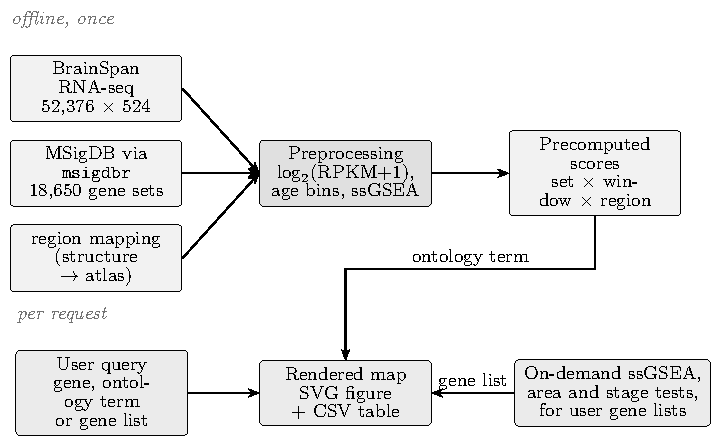
\includegraphics{fig1_architecture.pdf}
\caption{VEGABrain data flow. The top row runs once, offline; the bottom row
runs per request. Ontology queries are served from the precomputed score table,
whereas a user-submitted gene list triggers a fresh ssGSEA run over all 524
samples and, on request, the area and stage tests of Section~\ref{sec:tests}
against 4{,}000 expression-matched random gene sets.}
\label{fig:arch}
\end{figure}

%%==================================================================%%
\section{Results}\label{sec:results}
%%==================================================================%%

VEGABrain offers three query modes---a single gene, a precomputed ontology term,
or a user-submitted gene list---on a single working page.
All three produce the same four-panel, five-window
figure at either region granularity (Section~\ref{sec:mapping}), and a
reference map labelled by region name is available so that unfamiliar atlas
parcels can be identified. In gene-list mode the tests of
Section~\ref{sec:tests} add marks to the map and a developmental-stage panel
beside it. We illustrate each mode with a case
whose developmental behaviour is independently established, so that the maps
can also be judged for biological face validity.

\subsection{Single-gene maps}

Gene mode renders the mean $\log_2(\mathrm{RPKM}+1)$ of any gene in the matrix
per region and developmental window, on a fixed colour scale bounded at 6, so
that maps for different genes are directly comparable rather than each being
auto-scaled to its own range. Oligodendrocyte and myelination markers
(\emph{SOX10}, \emph{MBP}, \emph{PLP1}) should be low prenatally and rise
sharply in the child and adult windows as myelination proceeds;
Figure~\ref{fig:gene} shows \emph{SOX10}.

\subsection{Gene-set maps}

Ontology mode returns the mean ssGSEA score of any of the 18{,}650 precomputed
gene sets per region and window (Figure~\ref{fig:ontology}). This is the
composite layer described in Section~\ref{sec:ssgsea}, and it is what
distinguishes VEGABrain from a gene-at-a-time browser: a single map summarises
the coordinated behaviour of tens to hundreds of genes. The member genes of the
selected set are listed alongside the map, so the composition of any score is
inspectable. Astrocytes are generated after neurons, once cortical neurogenesis
gives way to gliogenesis \citep{Rowitch2010}, so
\texttt{GOBP\_ASTROCYTE\_DEVELOPMENT} should rise late in prenatal development.
Its map peaks in the third trimester, in cortex and subcortex alike
(Figure~\ref{fig:ontology}a). The composite score is informative here: the
individual genes of the term are noisy across 28 sparsely sampled parcels,
whereas the ssGSEA summary of its 42 genes is not. Submitting those genes in
gene-list mode (Supplementary Table~2) tests the reading directly (Figure~\ref{fig:ontology}b): against
random genes of the same expression level, the term is higher in the third
trimester (whole-brain $z = 6.1$; neocortex $4.7$, cerebellum $4.3$) and lower in
the first ($z = -2.6$). The hippocampus, amygdala, striatum and thalamus show the
same third-trimester peak ($z = 4.6$ to $5.9$) but cannot be tested there, as
each was sampled from only two donors in that window. The example also shows why
the stage test is needed. Because the term peaks everywhere at once, neither
area test, both of which compare areas within a window, marks any area in the
third trimester; the peak is a matter of when, not where.

\subsection{User-submitted gene lists}

In gene-list mode, a pasted list of symbols is validated and scored on demand
(Figures~\ref{fig:autism} and~\ref{fig:organoid}). Symbols absent from the matrix are listed back to
the user explicitly, so a map is never quietly computed on a subset of what was
submitted. This is the path from an external result to anatomy: the output of a
differential expression analysis, a co-expression module, or a disorder risk
panel can be mapped across development directly, without the user preparing
data or writing code. GABAergic interneuron markers (\emph{GAD1}, \emph{GAD2},
\emph{SLC32A1}) should be present from the second trimester onward with
subcortical and then cortical distribution. In addition to entering genes,
for each entry, the researcher can add a logFC value of their choice. The process can simulate 
how that variation in expression might impact the developmental process; the
tests then treat the up- and down-regulated genes separately, since the two
halves of a signature can belong to different areas or stages.

\subsection{Where and when: testing a gene list}\label{sec:showcase}

Figure~\ref{fig:autism} applies the three tests to a list whose developmental
answer is known from independent work: the 262 genes of the Human Phenotype
Ontology term \texttt{HP\_AUTISM} that are present in BrainSpan (Supplementary
Table~2). Autism risk
genes converge on mid-fetal cortical development
\citep{Willsey2013,Parikshak2013}. The marker test, drawn on the map
(Figure~\ref{fig:autism}a), asks which areas' specific genes the list contains,
and names them (Figure~\ref{fig:autism}c). The list holds 21 of the 490
neocortex markers of the third trimester, among them \emph{SATB2},
\emph{FOXG1}, \emph{TBR1} and \emph{SYNGAP1}, so every neocortical area sampled
in that window is marked; it also holds 5 of the 33 markers of the
second-trimester anterior cingulate cortex, mostly progenitor and glial genes
(\emph{SOX2}, \emph{SOX3}, \emph{ATP1A2}). The stage test recovers the timing
from the list alone: the list peaks in the second trimester (whole-brain
$z = 3.4$; hippocampus, amygdala and striatum, $z = 3.6$ to $3.9$) and is lower
in the third trimester and in the child window (Figure~\ref{fig:autism}b). The score
test, the alternative mark for the same map, finds ten neocortical cells, in the
second trimester (primary motor and somatosensory cortex, inferolateral temporal
cortex), in the child window and in adulthood. The term is broader than a curated risk
list---it includes syndromic genes such as the Bardet--Biedl ciliopathy
family---so the effect sizes are moderate, yet the three tests agree on a
prenatal, cortical reading.

\subsection{A signature with fold changes: ethanol in cerebral organoids}\label{sec:organoid}

A list can also carry the log2 fold changes of a differential-expression
result. \citet{Arzua2020} exposed two-month-old cerebral organoids, derived from
human induced pluripotent stem cells, to 50\,mM ethanol for 6\,h, and report 199
genes changed more than twofold ($P < 0.05$), 162 up and 37 down. Submitting
that table as published, with signed log2 fold changes (Supplementary
Table~2), gives a weighted map of
the 173 genes found in BrainSpan, 141 up and 32 down
(Figure~\ref{fig:organoid}). Cerebral organoids of this age resemble the early
and mid-fetal neocortex \citep{Camp2015,Gordon2021}, and the stage test places
the signature there with no information from the experiment: it is higher in
the first and second trimesters (whole-brain $z = 3.2$ and $4.9$), in every
region in the second trimester (the cerebellum resting on one donor), and lower
in the third trimester and in the child window ($z = -6.4$ and $-2.4$, both resting on
one donor at the whole-brain level; Figure~\ref{fig:organoid}b). The genes
ethanol raised carry this result (whole-brain $z = 3.3$ and $4.8$ in the first
two trimesters), while the 32 it lowered peak in no window. The score test marks
19 cells, all of them neocortical areas, in the first and second trimesters and
after birth (Figure~\ref{fig:organoid}a): within each window, the signature
stands out in the cortex rather than in subcortical structures. The marker test
agrees, placing raised genes such as \emph{MEF2C}, \emph{RORB} and
\emph{KCNV1} among the neocortex markers of all five windows.

%%------------------------------------------------------------------%%
%% Figures 2-5 (placeholders in this draft -- see IMPLEMENTATION.md)
%%------------------------------------------------------------------%%

\begin{figure}[htbp]
\centering
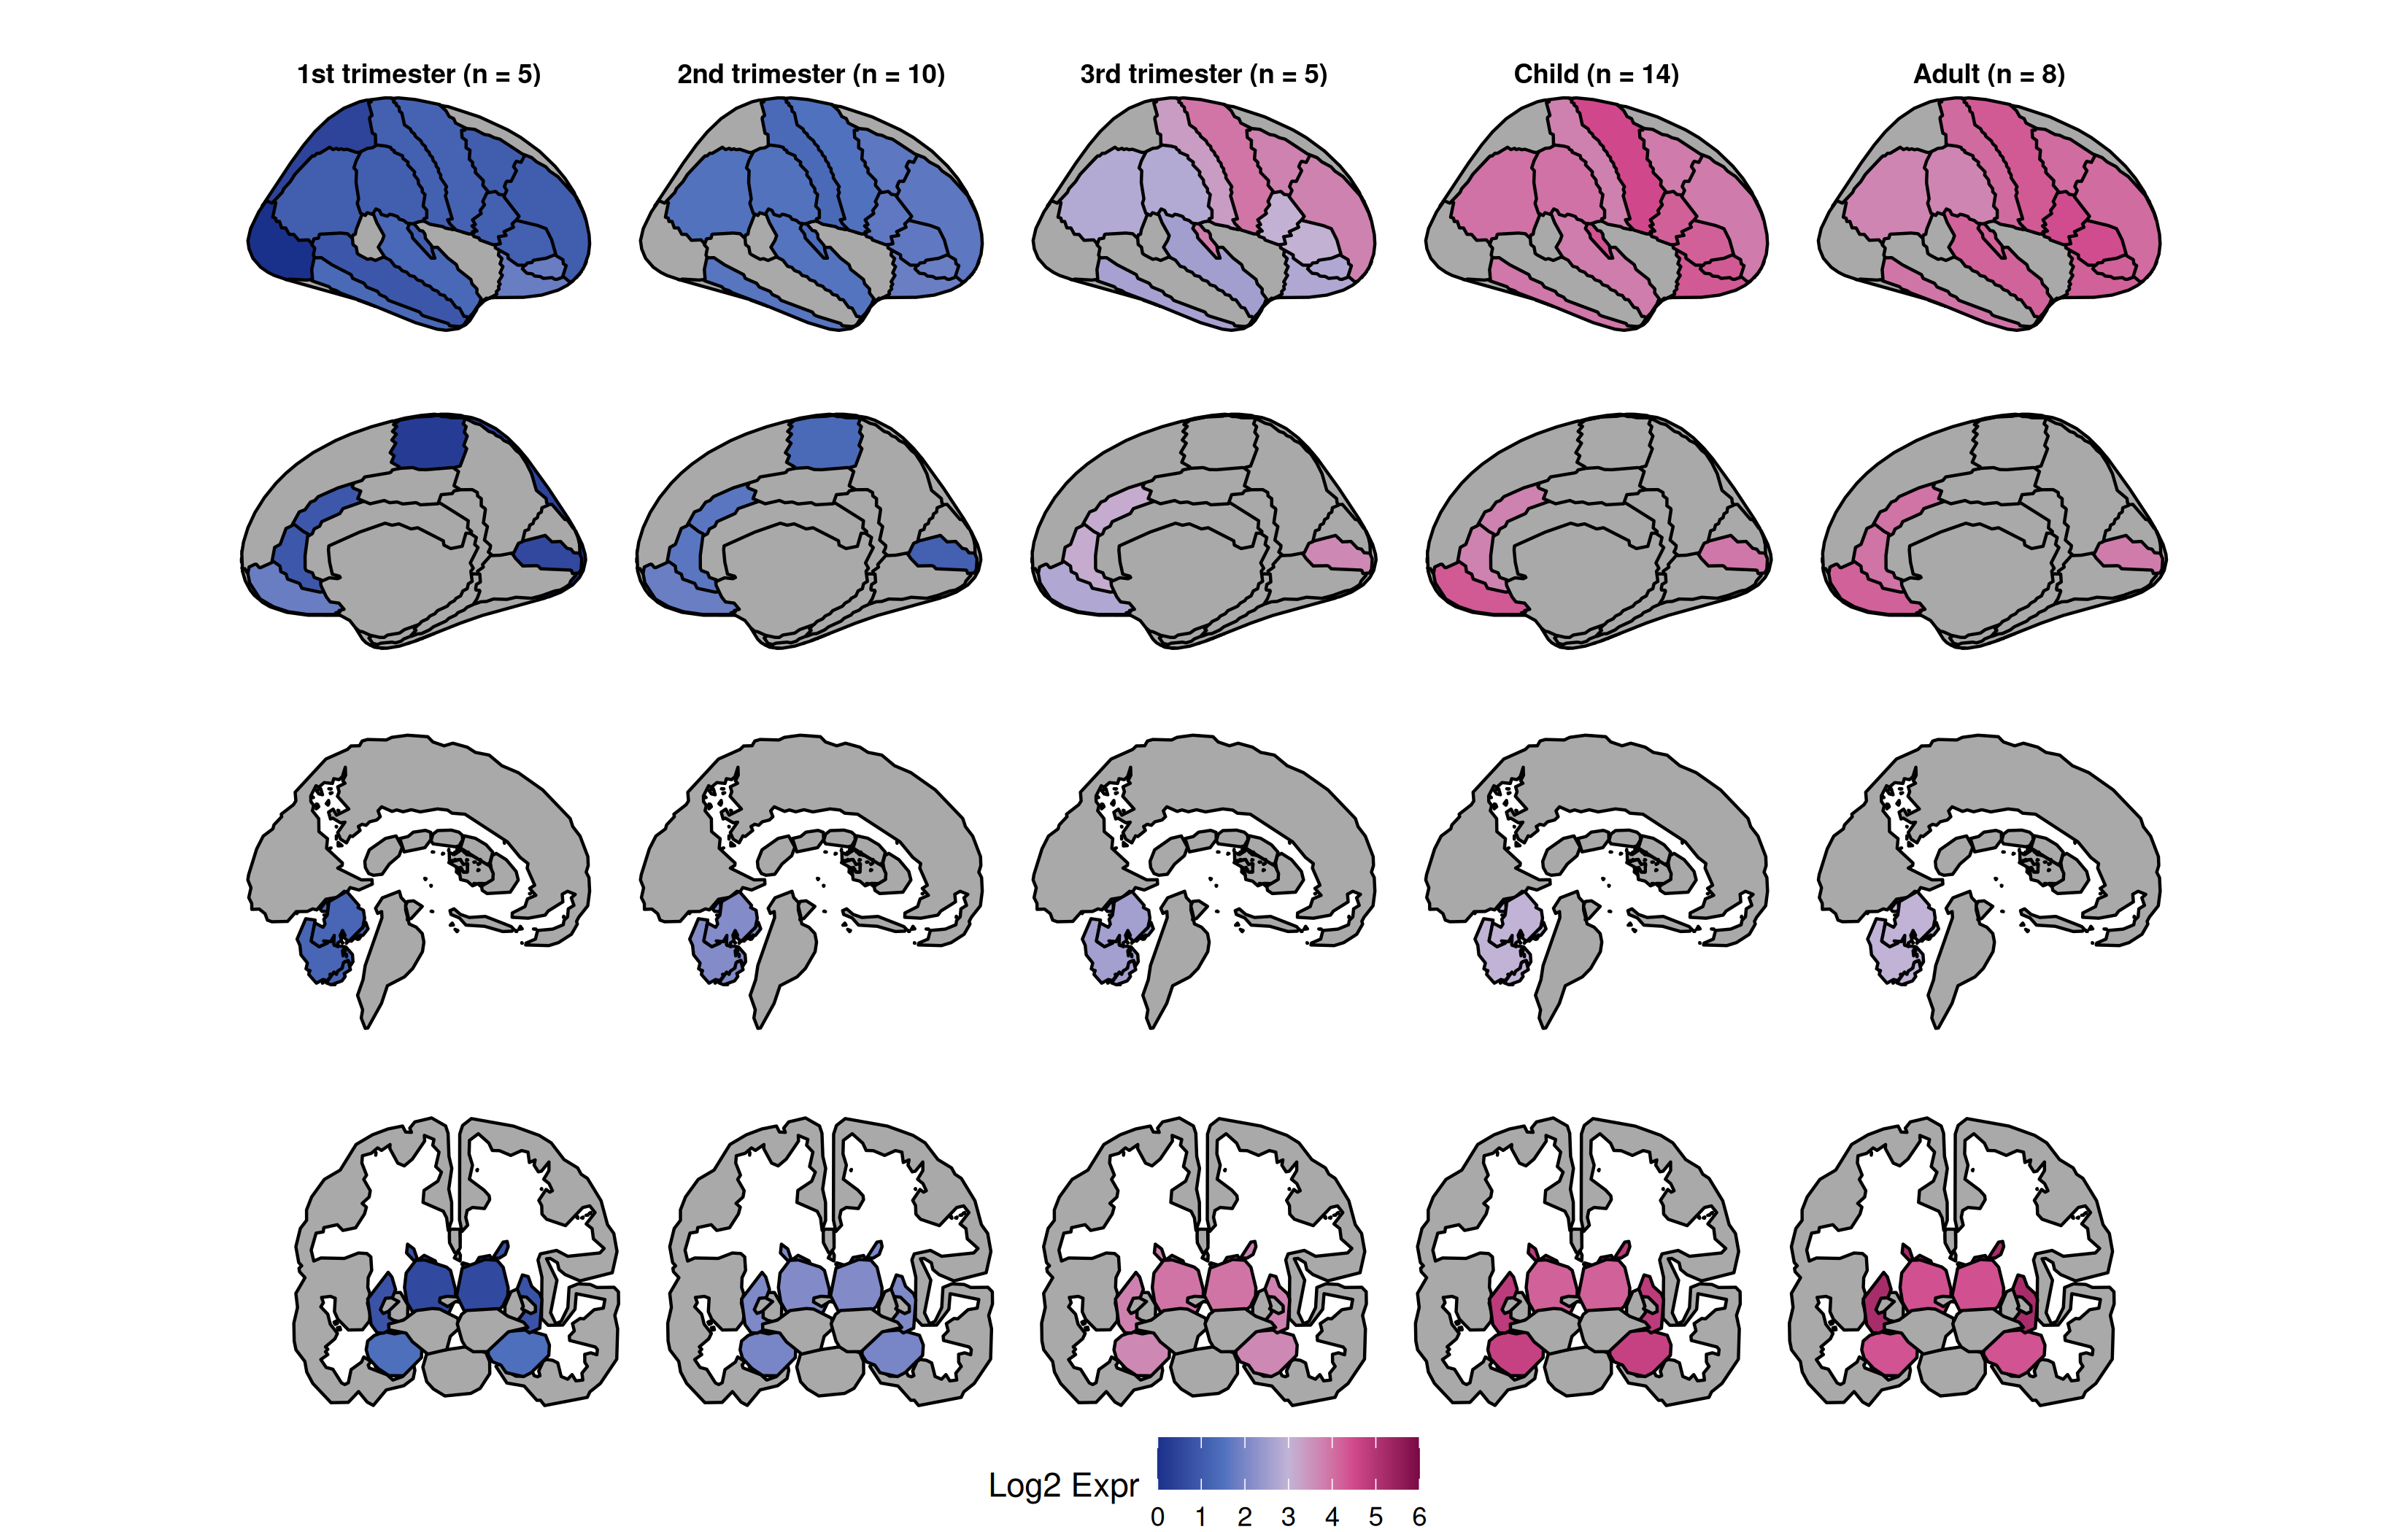
\includegraphics[width=\textwidth]{fig2_gene_sox10.png}
\caption{Single-gene mode. Mean $\log_2(\mathrm{RPKM}+1)$ for \emph{SOX10}
across the five developmental windows (columns) in four views (rows): right
lateral cortex and right medial cortex on the Desikan--Killiany parcellation,
and subcortical structures in sagittal and coronal section on the \texttt{aseg}
segmentation. Grey indicates regions with no BrainSpan sample in that window.}
\label{fig:gene}
\end{figure}

\begin{figure}[htbp]
\centering
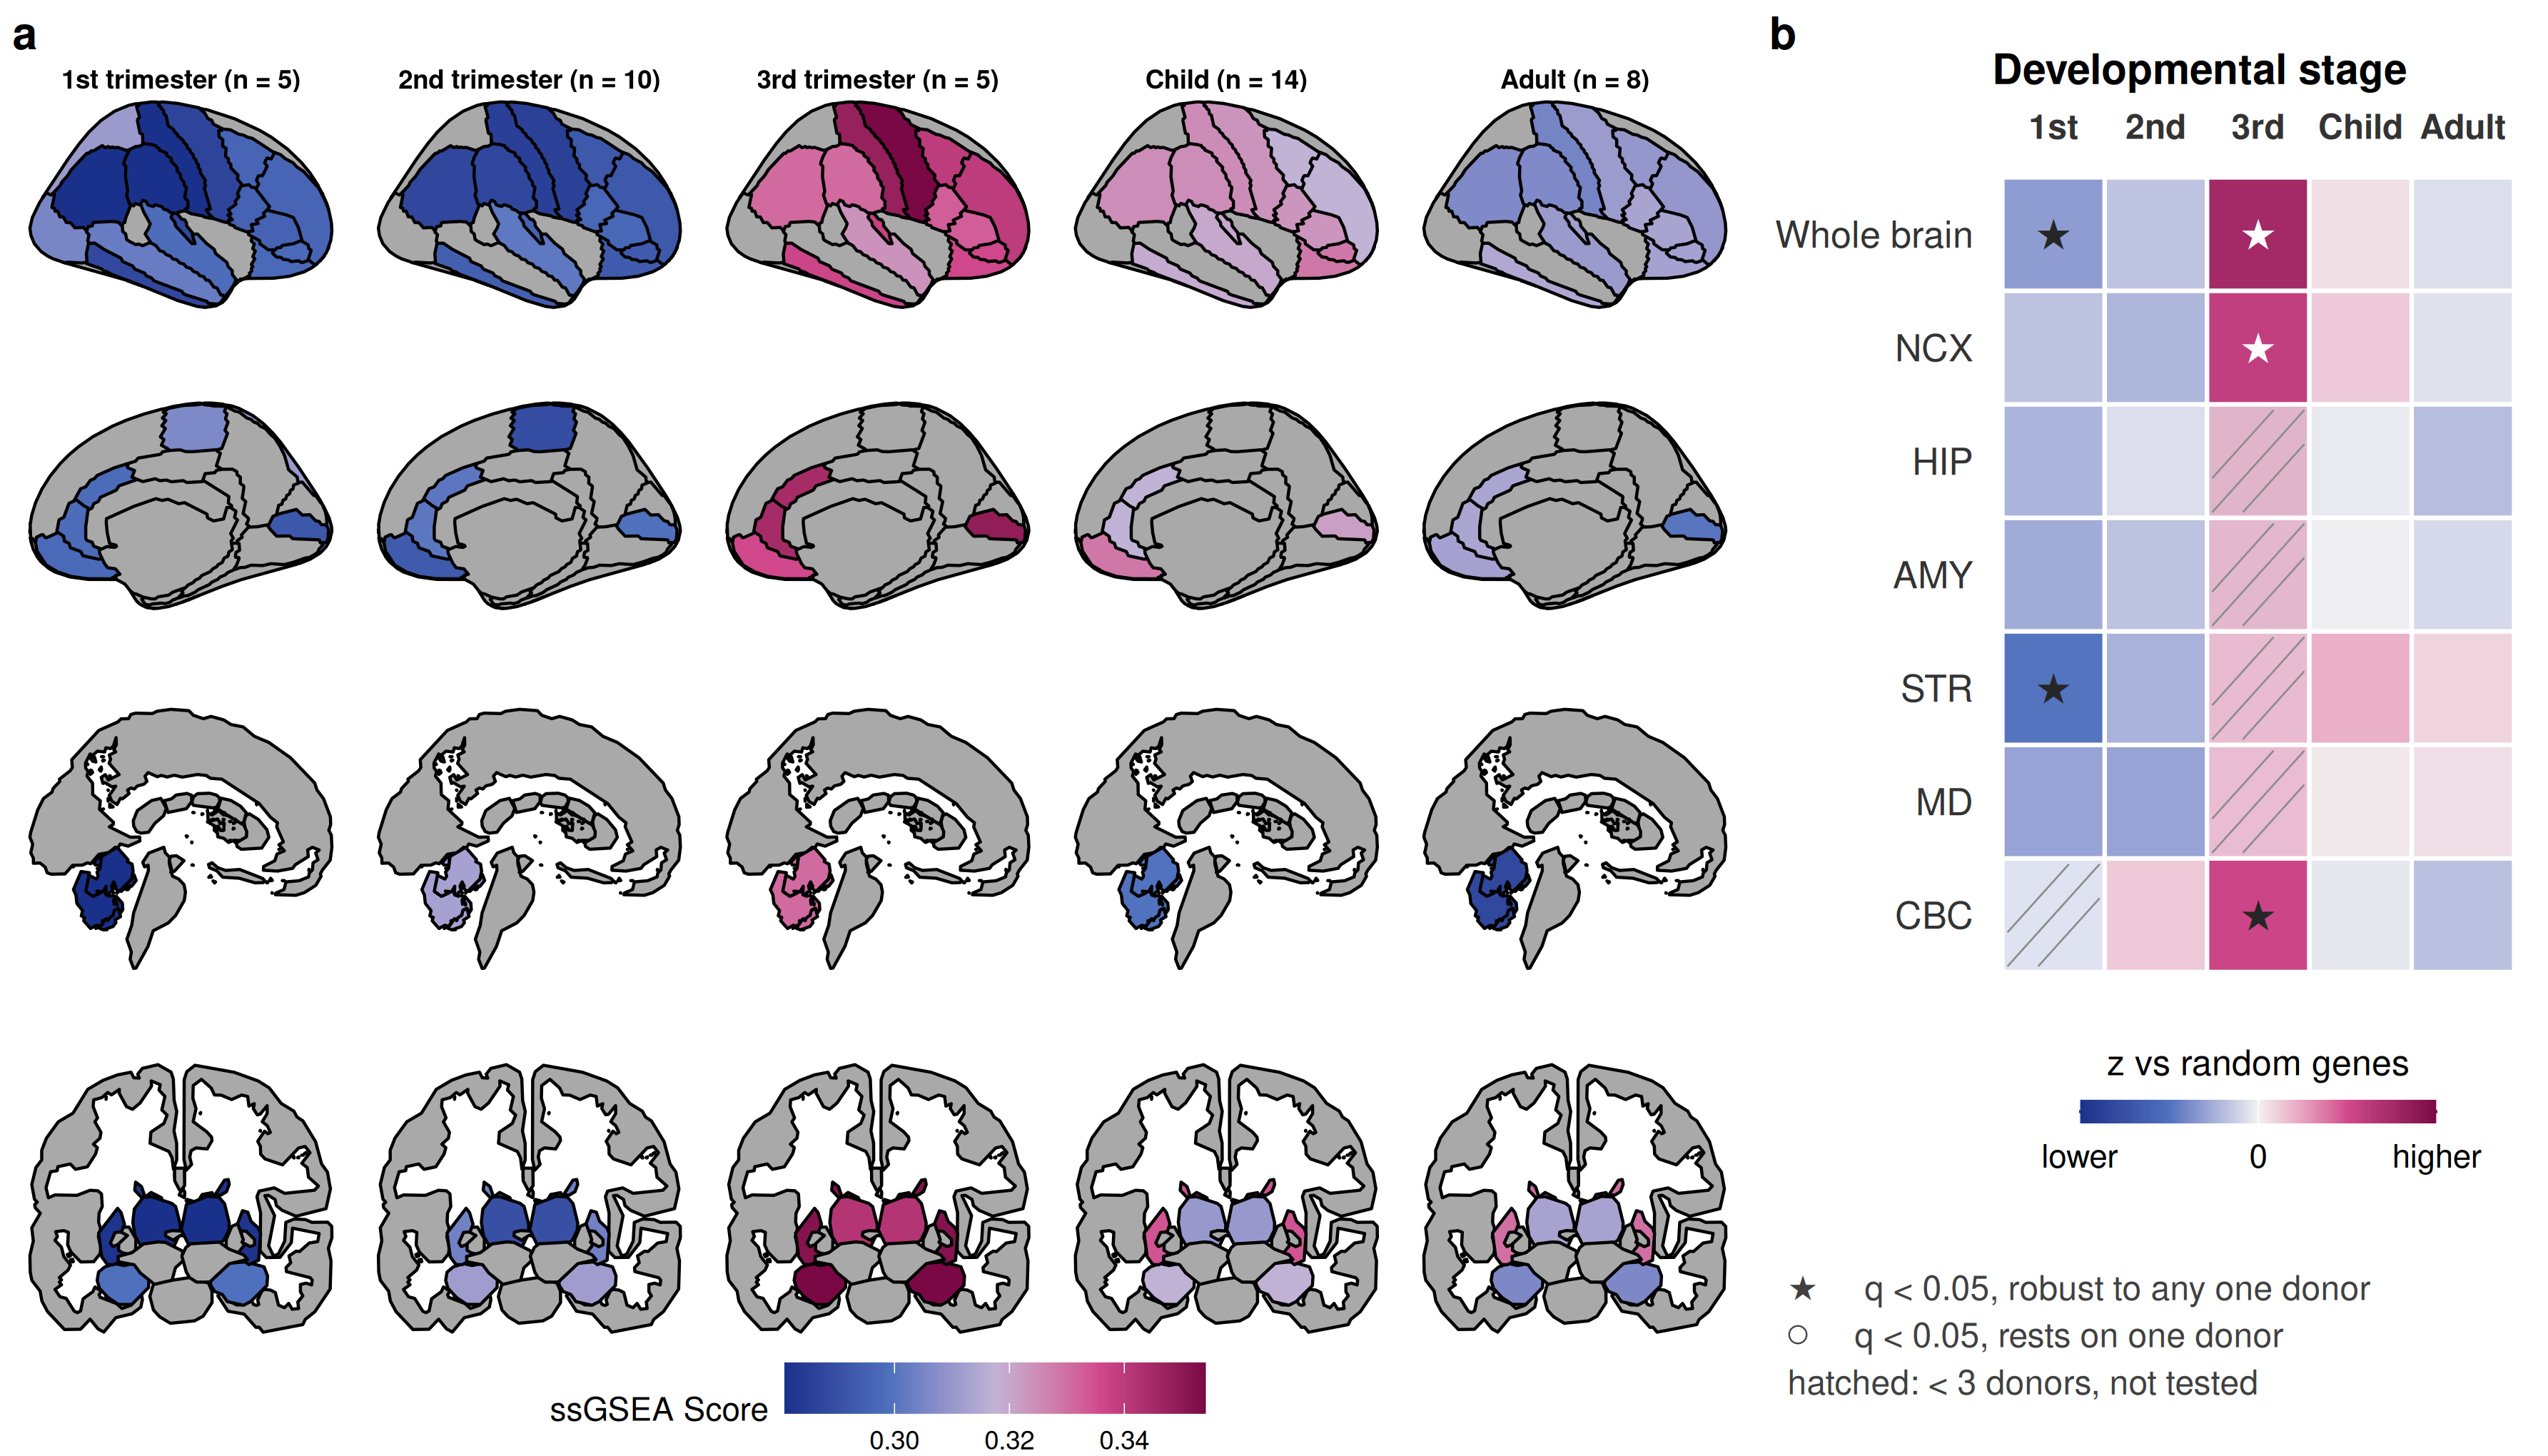
\includegraphics[width=\textwidth]{fig3_ontology.png}
\caption{Ontology mode. (a) Composite ssGSEA score for
\texttt{GOBP\_ASTROCYTE\_DEVELOPMENT} across development. The score
summarises every gene in the term into one value per region and window; the same
term can be viewed at micro granularity (28 atlas parcels) or macro granularity
(six anatomical groupings). (b) Developmental-stage test of the term's 42 genes
(Section~\ref{sec:tests}), for the whole brain and the six PsychENCODE regions.
Colour is $z$ against 4{,}000 expression-matched random gene sets, centred over
the five windows; a star marks $q < 0.05$ that survives leaving out any one
donor, a ring $q < 0.05$ resting on one donor, and hatching a cell with fewer
than three donors, which is not tested. The term peaks in the third trimester in
every region, but only the neocortex and the cerebellum have enough donors in
that window to be tested.}
\label{fig:ontology}
\end{figure}

\begin{figure}[htbp]
\centering
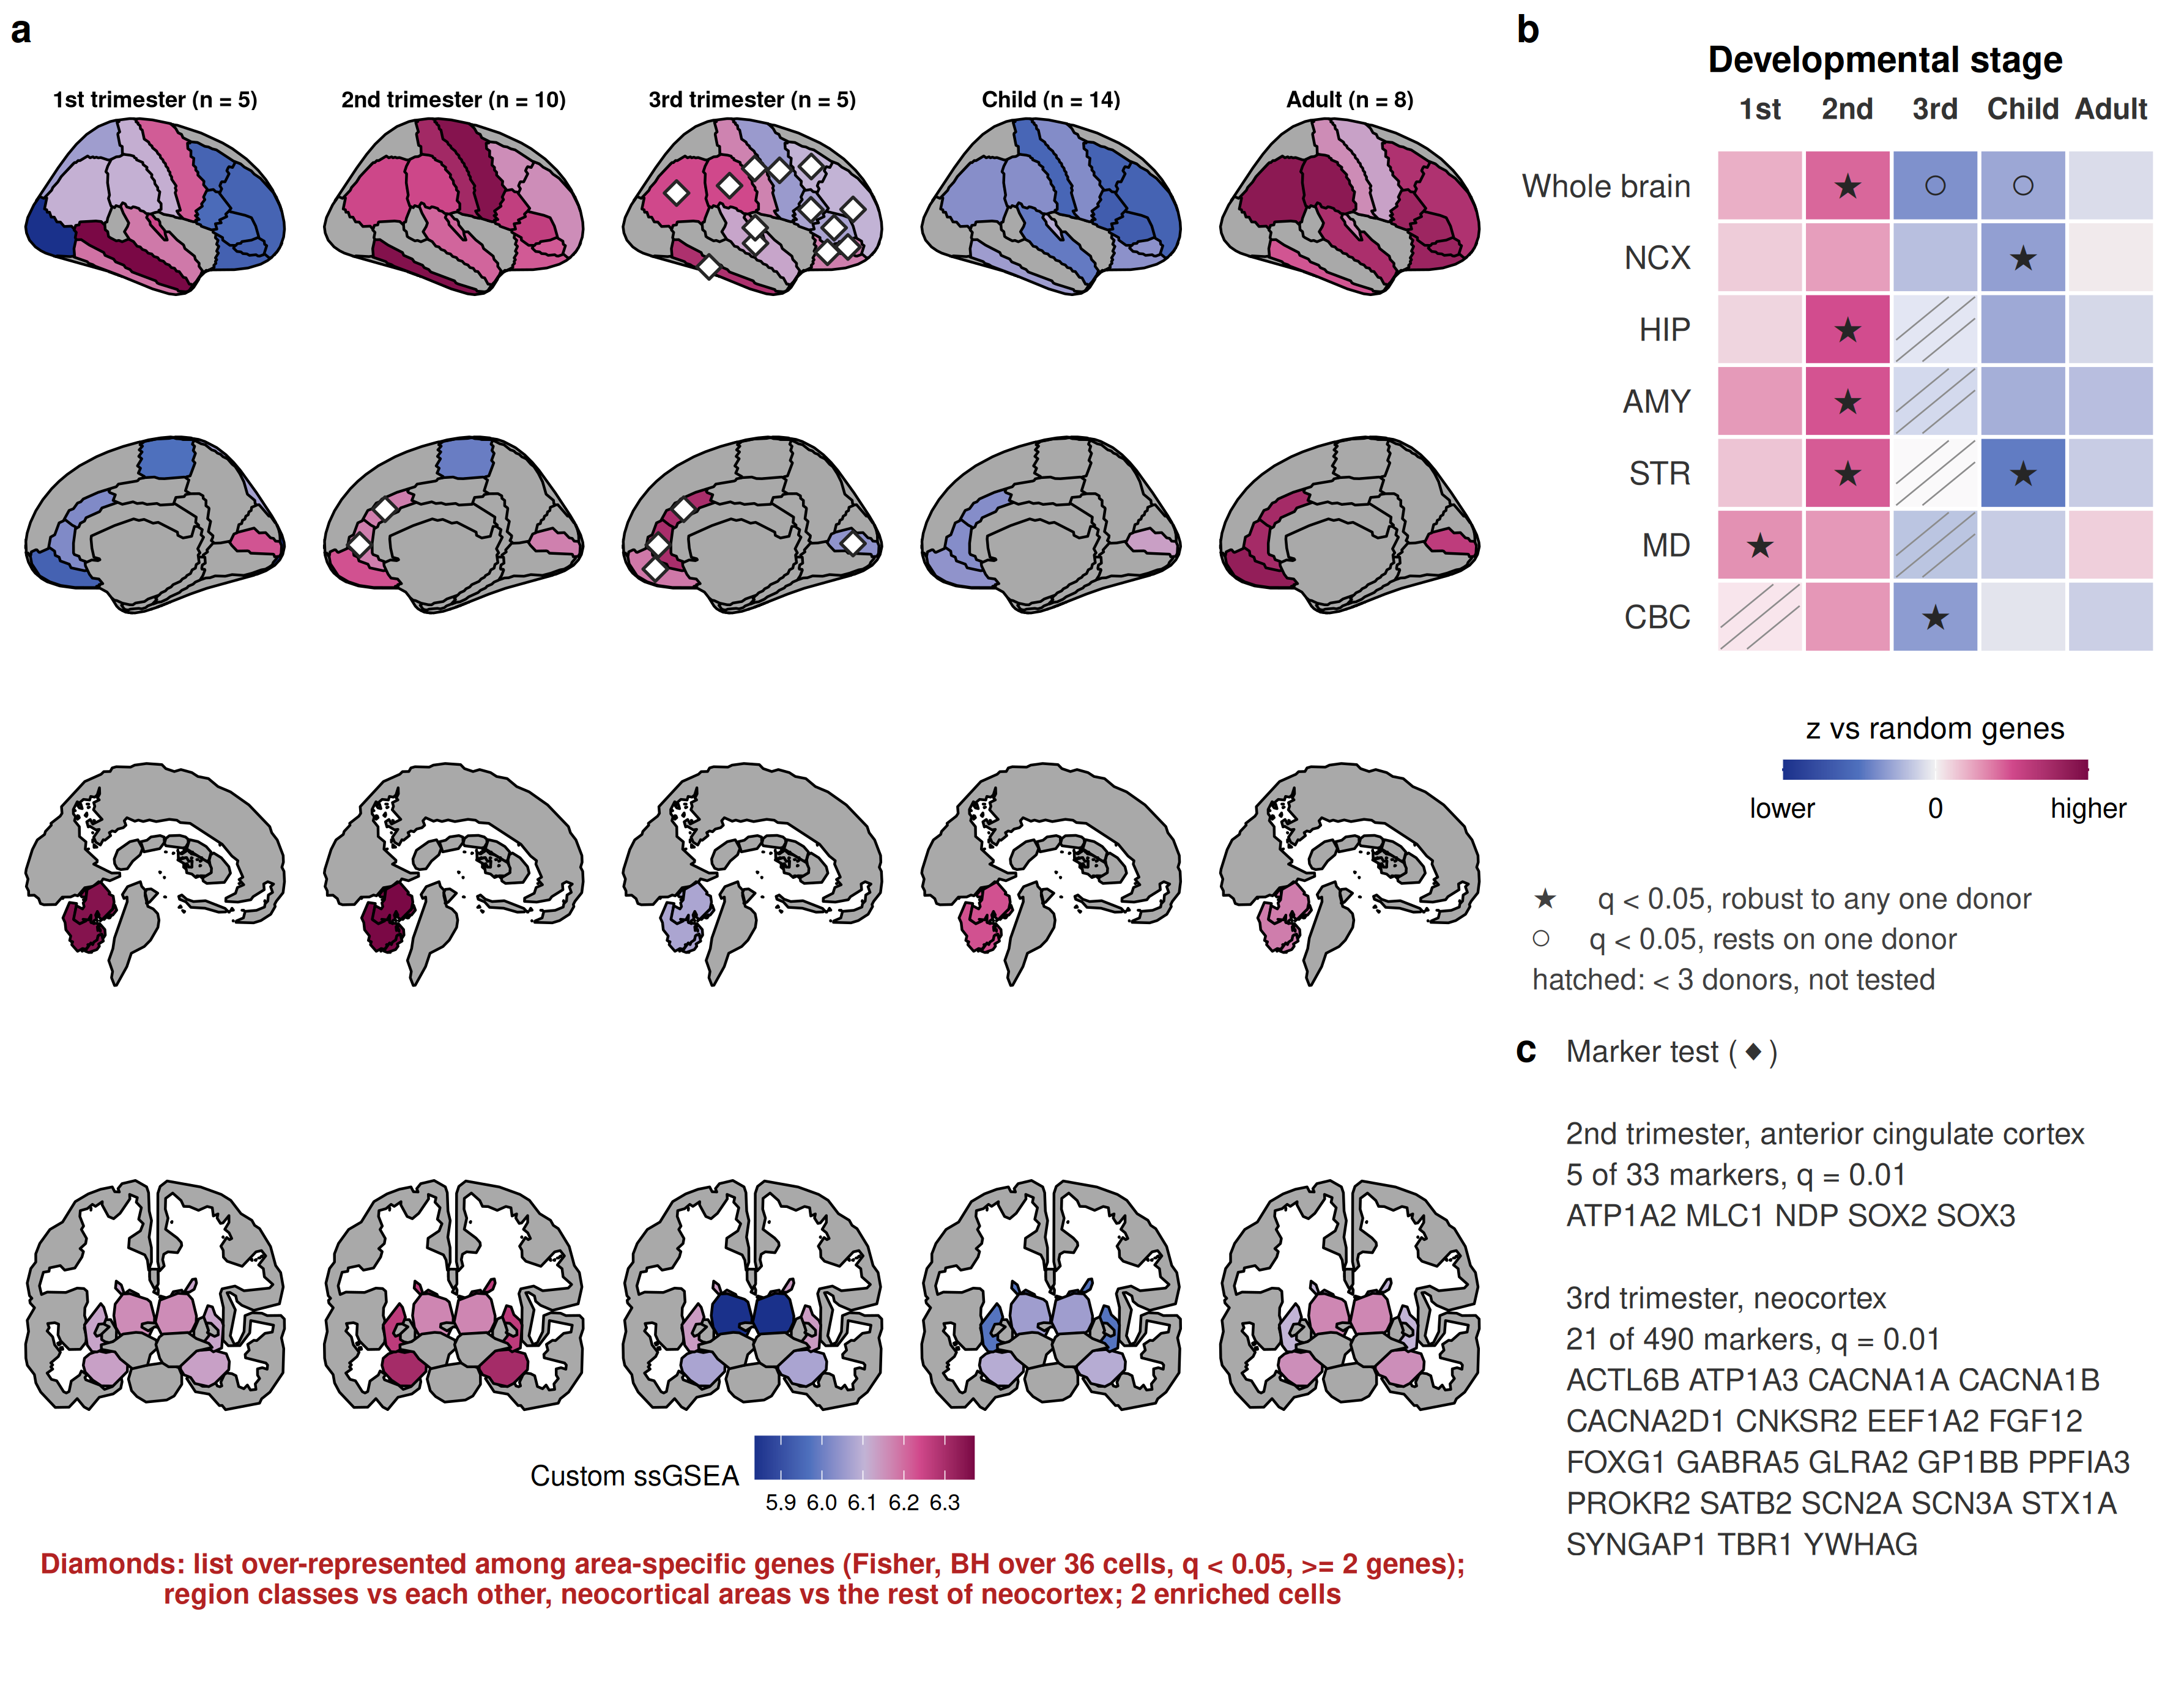
\includegraphics[width=\textwidth]{fig4_autism.png}
\caption{Where and when a gene list is enriched: the 262 genes of
\texttt{HP\_AUTISM} found in BrainSpan. (a) ssGSEA map with the marker test:
diamonds mark the areas whose specific genes are over-represented in the list
(one-sided Fisher test against \texttt{limma} area markers, $q < 0.05$, at least
two shared genes). A hit for the neocortex as a whole, here in the third
trimester, marks every neocortical area sampled in that window.
(b) Developmental-stage test, as in Figure~\ref{fig:ontology}b: the list peaks
in the second trimester, as autism risk genes are known to
\citep{Willsey2013,Parikshak2013}. (c) The cells marked in (a), with the shared
genes.}
\label{fig:autism}
\end{figure}

\begin{figure}[htbp]
\centering
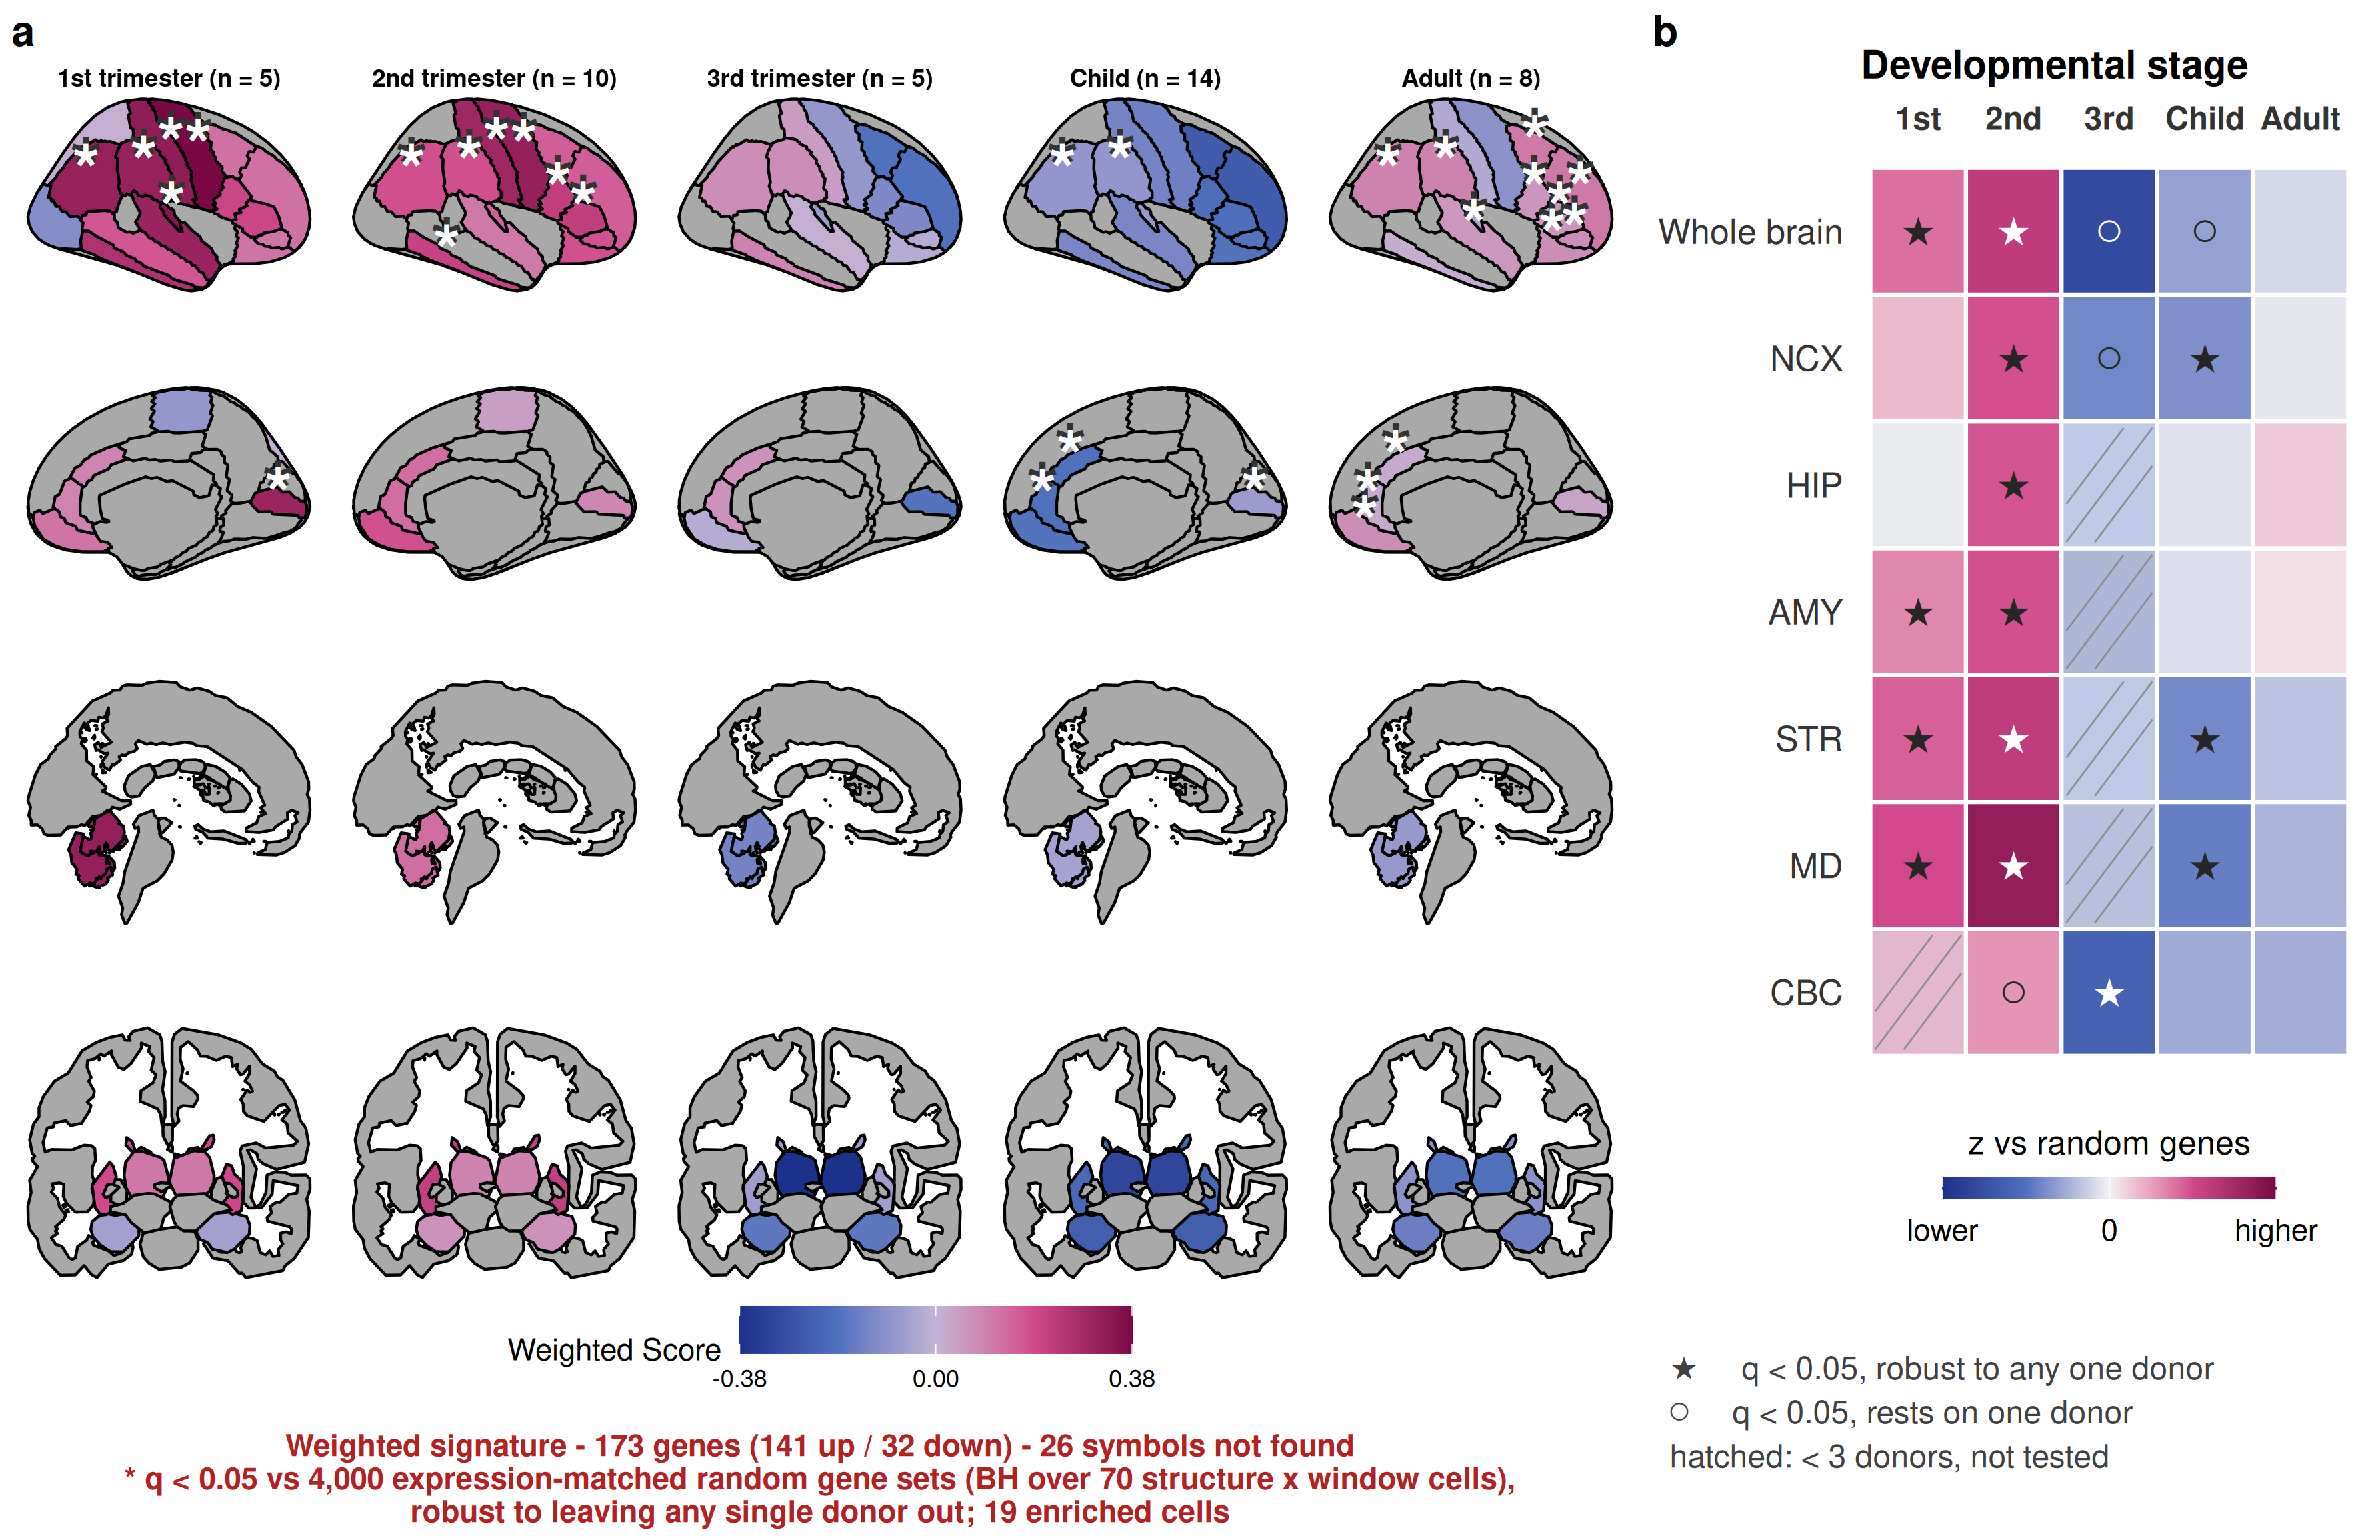
\includegraphics[width=\textwidth]{fig5_organoid.png}
\caption{A signature with fold changes: the genes changed by 6\,h of 50\,mM
ethanol in two-month-old human cerebral organoids \citep{Arzua2020}, submitted
with their signed log2 fold changes (173 of 199 genes found in BrainSpan; 141 up,
32 down). The list is a published differential-expression result, mapped without
local installation or coding. (a) Weighted score: magenta where the genes
ethanol raised are high relative to those it lowered, blue where the reverse
holds. Asterisks mark the score test: structures where the weighted score
exceeds that of 4{,}000 expression-matched random gene sets carrying the same
weights ($q < 0.05$, robust to leaving out any donor); all 19 are neocortical
areas. (b) Developmental-stage test of the weighted list, as in
Figure~\ref{fig:ontology}b: higher in the first and second trimesters, the
stage that organoids of this age resemble.}
\label{fig:organoid}
\end{figure}

%%------------------------------------------------------------------%%
%% Table 1 -- data summary
%%------------------------------------------------------------------%%
\begin{table}[htbp]
\centering
\caption{Data underlying VEGABrain.}\label{tab:data}
\begin{tabular}{@{}ll@{}}
\toprule
Property & Value \\
\midrule
Expression source        & BrainSpan RNA-Seq, Gencode v10 RPKM, gene-summarised \\
Matrix dimensions        & 52{,}376 genes $\times$ 524 samples \\
Transformation           & $\log_2(\mathrm{RPKM}+1)$; duplicate symbols dropped \\
Developmental windows    & 5 (see below) \\
\quad 1st trimester      & 5 donors, 8--12 pcw \\
\quad 2nd trimester      & 10 donors, 13--21 pcw \\
\quad 3rd trimester      & 5 donors, 24--37 pcw \\
\quad Child              & 14 donors, 4 months--15 years \\
\quad Adult              & 8 donors, 18--40 years \\
Atlas parcels (micro)    & 28 (21 Desikan--Killiany cortical + 7 \texttt{aseg}) \\
Anatomical groups (macro)& 6 (frontal, parietal, temporal, occipital, subcortical, cerebellum) \\
Views per map            & 4 (DK lateral, DK medial, \texttt{aseg} sagittal, \texttt{aseg} coronal) \\
Gene sets scored         & 18{,}650 total \\
\quad GO biological process & 7{,}538 \\
\quad Human Phenotype Ontology & 5{,}793 \\
\quad GO molecular function & 1{,}872 \\
\quad Reactome           & 1{,}839 \\
\quad GO cellular component & 1{,}080 \\
\quad BioCarta           & 292 \\
\quad KEGG (legacy)      & 186 \\
\quad MSigDB hallmark    & 50 \\
\botrule
\end{tabular}
\end{table}

%%------------------------------------------------------------------%%
%% Table 2 -- calibration of the significance tests
%%------------------------------------------------------------------%%
\begin{table}[htbp]
\centering
\caption{Calibration of the significance tests: share of lists with at least
one marked cell.}\label{tab:tests}
\footnotesize
\setlength{\tabcolsep}{4pt}
\begin{tabular}{@{}lccccc@{}}
\toprule
& \multicolumn{3}{c}{Random lists (no signal)} & Expression-matched & Real MSigDB \\
\cmidrule(lr){2-4}
Test & 15 genes & 50 genes & 200 genes & swaps (no signal) & sets \\
\midrule
Score (per structure)          & 2.0\% & 3.5\% & 4.0\% & ---   & 36\% \\
Marker (per class or area)     & 1.8\% & 1.8\% & 1.8\% & 3.0\% & 15\% \\
Stage, whole brain             & 3.0\% & 3.0\% & 4.3\% & 2.3\% & 44\% \\
Stage, six regions             & 2.5\% & 2.5\% & 3.5\% & 2.5\% & 46\% \\
\botrule
\end{tabular}
\footnotetext{A marked cell is one that passes Benjamini--Hochberg correction at
$q < 0.05$ and, for the score and stage tests, the leave-one-donor-out check.
Random lists: 200 per size (score test, 2{,}000 random sets each), 500 (marker
test) and 300 or 200 (stage test, whole brain or regions, 1{,}000 random sets
each). Random lists of 50 genes with log2FC weights drawn from
$\mathcal{N}(0, 1)$ gave 3.0\% (score, 100 lists), 0.6\% (marker) and 3.0\%
(stage). Real sets: 15 to 300 genes found in the data, 200 sets (score) or 300
(marker, stage). Scripts: \texttt{stats/validate\_stats.R},
\texttt{stats/validate\_markers.R} in the repository.}
\end{table}

%%==================================================================%%
\section{Discussion}\label{sec:discussion}
%%==================================================================%%

VEGABrain lowers the cost of asking a spatial question of the developing human
transcriptome from a small project to a few seconds in a browser. The composite enrichment layer extends the same reasoning to the
unit that modern analyses actually produce---a gene set---and the on-demand mode
means a user's own list is a first-class input rather than something the tool's
authors had to anticipate. The significance tests take the last step: they turn
a map into a result, by marking where and when a list stands out against random
genes of the same expression level, and by naming the genes behind each area
hit.

\subsection{Relation to existing tools}\label{sec:comparison}

Table~\ref{tab:compare} positions VEGABrain against the tools a researcher would
otherwise reach for. The comparison is deliberately along axes of \emph{what the
user must supply}, not of raw capability: each of these tools is stronger than
VEGABrain in its own domain, and the point is that none of them closes the
particular path VEGABrain is built for---from a gene set to a scored,
parcellated map of the developing brain, in a browser.

\begin{table}[htbp]
\centering
\caption{VEGABrain relative to comparable tools. \checkmark{} = supported,
--- = not supported or out of scope.}\label{tab:compare}
\footnotesize
\setlength{\tabcolsep}{4pt}
\begin{tabular}{@{}p{44mm}ccccc@{}}
\toprule
& Developmental & Anatomical & Gene-set & Custom list & No install \\
& axis & rendering & scoring & input & required \\
\midrule
VEGABrain (this work)             & \checkmark & \checkmark & \checkmark & \checkmark & \checkmark \\
BrainSpan portal \citep{BrainSpan2011} & \checkmark & ---   & ---        & ---        & \checkmark \\
Allen browsers \citep{Sunkin2013} & ---   & \checkmark & ---     & ---        & \checkmark \\
BrainScope \citep{Huisman2017}         & \checkmark & \checkmark & ---   & \checkmark & \checkmark \\
SMDB \citep{Cao2023}                   & ---        & \checkmark & ---   & ---        & \checkmark \\
\texttt{ggseg} \citep{Mowinckel2020}   & ---        & \checkmark & ---   & \checkmark & --- \\
\texttt{neuromaps} \citep{Markello2022}& ---        & \checkmark & ---   & \checkmark & --- \\
\texttt{abagen} \citep{Markello2021}   & ---        & \checkmark & ---   & \checkmark & --- \\
\texttt{cerebroViz} \citep{Bahl2017}   & \checkmark & \checkmark & ---   & \checkmark & --- \\
Programmatic plotting guides \citep{Chopra2023} & --- & \checkmark & --- & \checkmark & --- \\
Enrichr \citep{Chen2013,Kuleshov2016}  & ---        & ---        & \checkmark & \checkmark & \checkmark \\
\texttt{VoxHunt} \citep{Fleck2021}     & \checkmark & \checkmark & ---   & \checkmark & --- \\
\texttt{ABAEnrichment} \citep{Grote2016} & \checkmark & ---   & ---   & \checkmark & --- \\
\botrule
\end{tabular}
\footnotetext{``Developmental axis'' means the tool natively presents variation
across prenatal-to-postnatal time. ``Anatomical rendering'' means values are
drawn onto a picture of the brain, in whatever form the tool adopts---a
parcellated surface, a slice choropleth or a three-dimensional point cloud.
``Gene-set scoring'' means it produces a composite per-sample score for a set of
genes rather than plotting genes individually; a tool that displays the mean
expression of a set, or that hands the set to an external enrichment server,
does not qualify. ``Custom list input'' means the user may supply their own
genes or their own per-region values.}
\end{table}

As noted in the Introduction, the portals are gene-at-a-time and the
programmatic tools take a value per region as \emph{input}, leaving the user to
obtain, preprocess and map the developmental expression data themselves.
\texttt{cerebroViz} \citep{Bahl2017} is the closest of them in intent, having
been written for spatiotemporal brain data specifically and shipping region
vocabularies for BrainSpan, GTEx \citep{GTEx2013} and Roadmap Epigenomics
\citep{Roadmap2015}; it nonetheless remains
a drawing layer over a matrix the user provides, carries no expression data of
its own, and computes no enrichment. The same qualification applies to the
code-first route as a whole. \citet{Chopra2023} argue for it persuasively and
lower its cost with a survey of the available packages and a generator for
template plotting code, but a guide to writing the code does not remove the
prerequisites the code still has: a working R or Python environment, a local
copy of the expression matrix, and a mapping from tissue nomenclature onto a
parcellation.

Among hosted resources, BrainScope \citep{Huisman2017} is the nearest neighbour
to VEGABrain, and the only other entry in Table~\ref{tab:compare} that is at
once web-based, developmental and willing to take a user's own gene set. The
abstraction differs, and with it the question answered. BrainScope arranges the
Allen adult and developing atlases as linked t-SNE maps of genes and samples,
localising samples anatomically through choropleths over selected slices, and
summarises a submitted set by its mean expression while delegating enrichment to
Enrichr \citep{Chen2013} and ToppGene \citep{Chen2009}. VEGABrain asks the narrower question of where a set sits
in a named parcellation, window by window, and answers it with a rank-based
composite score rather than a mean, drawn on the Desikan--Killiany and
\texttt{aseg} atlases that the imaging literature already uses. SMDB
\citep{Cao2023} is likewise hosted and likewise anatomical, but for a different
data type and species: it browses spatial transcriptomics sections against
Allen's mouse brain coordinate framework and reconstructs morphology in three
dimensions, with no human developmental axis and no gene-set layer.

Enrichr \citep{Chen2013,Kuleshov2016} performs the gene-set reasoning but
returns ranked term tables, with no anatomical or developmental dimension.
\texttt{VoxHunt} \citep{Fleck2021} maps expression signatures onto developmental
reference atlases, primarily to assign identity to \emph{in vitro} organoid
samples, and is an R package rather than a hosted service. VEGABrain occupies the
intersection the others leave open: hosted, developmental, parcellated, and
gene-set \emph{scored}.

Testing a gene set for regional or developmental enrichment has been done
before, though not in a hosted, anatomical tool. \texttt{ABAEnrichment}
\citep{Grote2016} tests gene sets for expression enrichment across the regions
and developmental stages of the Allen atlases, BrainSpan included, as an R
package that returns tables. The specificity index and the tissue-specific
expression analyses built on it \citep{Dougherty2010,Xu2014} ask, as VEGABrain's
marker test does, whether a list is over-represented among genes specific to a
region and developmental period. VEGABrain combines a test of that kind with a
competitive test on the composite score and with a test of developmental
timing, and draws all three on the same parcellated map for any list a user
pastes.

\subsection{Limitations}\label{sec:limitations}

Some limitations bound the interpretation of any map produced here, and the
interface is designed to keep them visible rather than to smooth them over.
First, donor support is small and uneven: each developmental window rests on 5
to 14 donors, and not every structure is sampled in every window. Donor counts
are printed in every facet label and unsampled regions are drawn in grey rather
than interpolated, and the tests of Section~\ref{sec:tests} leave cells with
fewer than three donors untested rather than test them. Even so, the third
trimester rests mostly on two donors, of 24 and 37 post-conception weeks, so a
third-trimester result often reads as ``near term'', and a contrast resting on
few donors deserves less weight than its $q$-value alone suggests. The many-to-one assignment of
BrainSpan structures to atlas parcels (Section~\ref{sec:mapping}) likewise means
that neighbouring parcels sharing a structure cannot differ.

Second, the data are bulk tissue. BrainSpan samples are dissected tissue, so a
regional value reflects both cell-intrinsic expression and cell-type
composition: a rise in an oligodendrocyte programme across development is as
consistent with more oligodendrocytes as with more transcription per cell.
Single-cell atlases resolve this and are the natural next data source.

Third, ssGSEA scores are built from within-sample ranks. Equation~\ref{eq:ssgsea}
yields a value that is comparable across samples for a fixed gene set, but not
across gene sets of different sizes and not on an absolute scale. Colour scales
for ontology maps are therefore free rather than fixed, and a score should be
read as a spatiotemporal pattern, not as a magnitude.

Fourth, the score and stage tests are competitive: they compare a list with
random genes of matched expression, which ignores the correlation among the
list's own genes \citep{Goeman2007,Wu2012}. A coherent programme therefore
passes more easily than random genes do, and because development dominates
brain expression, about four in ten curated gene sets peak in some window. Each
cell is reported with its effect size ($z$), which should be read alongside the
mark. The marker test inherits the bulk-tissue caveat in another form: cortical
areas converge after birth, so fewer area-specific genes are found and fewer
postnatal areas can be tested.

Future work follows directly from these bounds: incorporating single-cell and
single-nucleus developmental atlases, which would let the marker test speak of
cell types rather than tissue, testing against correlation-aware nulls, and
allowing user-supplied parcellations.

%%==================================================================%%
\section{Conclusion}\label{sec:conclusion}
%%==================================================================%%

VEGABrain makes the developmental human brain transcriptome, and the activity of
gene sets within it, visible anatomically without installation, coding or data
preparation, and it tests submitted gene lists for where and when they are
enriched against expression-matched random genes. Maps and their underlying tables are exportable, the
structure-to-atlas mapping is published rather than implied, and the source is
open. The tool is available at \url{https://mcblab.github.io/VEGABrain/}.

%%==================================================================%%
\backmatter
%%==================================================================%%

\bmhead{Supplementary information}

\textbf{Supplementary File 1} is the assignment of BrainSpan dissected
structures to atlas parcels used by VEGABrain (Section~\ref{sec:mapping}), as a
CSV table (\texttt{S1\_region\_mapping.csv}) with one row per
parcel--structure pair. Column
\texttt{region} is the Desikan--Killiany or \texttt{aseg} parcel as named by
\texttt{ggseg}; \texttt{structure\_name} is the BrainSpan structure whose
samples are averaged into that parcel; \texttt{macro\_regions} is the
macro-scale grouping (frontal, parietal, temporal or occipital lobe,
subcortical, or cerebellum). A parcel fed by two
structures appears on two rows (thalamus, cerebellum), and the thalamus is
listed under both \texttt{Thalamus} and \texttt{Thalamus Proper}, the names it
carries in different FreeSurfer \texttt{aseg} versions, so the table's 29
region names denote 28 parcels.

\textbf{Supplementary Table 2} (\texttt{S2\_signatures.xlsx}) gives every gene
signature used in this work, one tab per signature: the lists of
Figures~\ref{fig:ontology}, \ref{fig:autism} and~\ref{fig:organoid}
(\texttt{GOBP\_ASTROCYTE\_DEVELOPMENT}, \texttt{HP\_AUTISM} and the ethanol
signature of \citealp{Arzua2020}) and the positive controls of
Section~\ref{sec:tests} (eight striatal markers, \texttt{GOBP\_MYELIN\_ASSEMBLY},
\texttt{HALLMARK\_G2M\_CHECKPOINT} and \texttt{HALLMARK\_E2F\_TARGETS}).
Column \texttt{gene} is what was submitted to the gene-list mode, and
\texttt{found\_in\_BrainSpan} marks the symbols present in the expression
matrix, which are the only ones that enter a map or a test. The tab for
\citet{Arzua2020} keeps the source table's fold change, direction, $P$ and
false discovery rate, and the signed log2 fold change submitted with each gene.
A README tab gives each signature's source and the counts quoted in the text.

\bmhead{Acknowledgements}

We thank the Allen Institute for Brain Science and the BrainSpan consortium for
making the developmental transcriptome openly available, and the maintainers of
\texttt{ggseg}, \texttt{GSVA} and \texttt{msigdbr}, on which this work depends.
The authors would like to thank NPAD / UFRN for computational resources.

\section*{Declarations}

\bmhead{Funding}
% TODO(authors): funding sources and grant numbers, or an explicit statement
% that no funding was received.
J.V.F.C. was financed by the Brazilian Agency Coordination for the Improvement of Higher Education Personnel (CAPES – Portuguese: Coordenação de Aperfeiçoamento de Pessoal de Nível Superior - Brasil (CAPES)- (project number 88887.002655/2024-00)

\bmhead{Competing interests}
The authors declare no competing interests.

\bmhead{Ethics approval and consent to participate}
Not applicable. This study analyses publicly released, de-identified data from
the BrainSpan Developmental Transcriptome and involved no new human subjects.

\bmhead{Data availability}
The expression data analysed here are the BrainSpan Developmental Transcriptome
RNA-Seq Gencode v10 summarised-to-genes release \citep{BrainSpan2011,Li2018},
publicly available at
\url{https://www.brainspan.org}. Gene sets were obtained from MSigDB through the
\texttt{msigdbr} R package. The derived per-region, per-window score tables
served by VEGABrain are downloadable as CSV directly from the application.

\bmhead{Code availability}
VEGABrain is open source at \url{https://github.com/MCBLab/VEGABrain}. The
application is deployed at \url{https://mcblab.github.io/VEGABrain/}; its public
HTTP API is documented in the repository.
% TODO(authors): add the licence and a Zenodo DOI for the archived release.

\bmhead{Author contributions}
% TODO(authors): complete using CRediT roles.
IM: Formal analysis, Methodology, Visualization, Writing – review and editing. 
JVFC: Formal analysis, Writing – review and editing. 
DMC: Conceptualization, Data curation, Investigation, Supervision, Writing – original draft, Writing – review and editing.

\bigskip

\bibliography{references}

\end{document}
